\documentclass[11pt,a4paper]{article}
\usepackage[margin=1in]{geometry}
\usepackage{graphicx}
\usepackage{booktabs}
\usepackage{float}
\usepackage{amsmath}
\usepackage{url}
\usepackage{hyperref}

\title{\textbf{Medical Image Analysis using UNet}}
\author{Louis Etienne Kusno 2025403026}
\date{}

\begin{document}

\maketitle

\section{Introduction}
Medical image analysis is a critical field in healthcare. In this project the goal was to use a neural network to detect regions of legion in brain MRI images.

A UNet architecture was used for this task. UNet is a convolutional neural network that was originally designed for biomedical image segmentation \cite{ronneberger2015u}. It has a U-shaped architecture that consists of a contracting path to capture context and a symmetric expanding path that enables precise localization.

\begin{figure}[H]
    \centering
    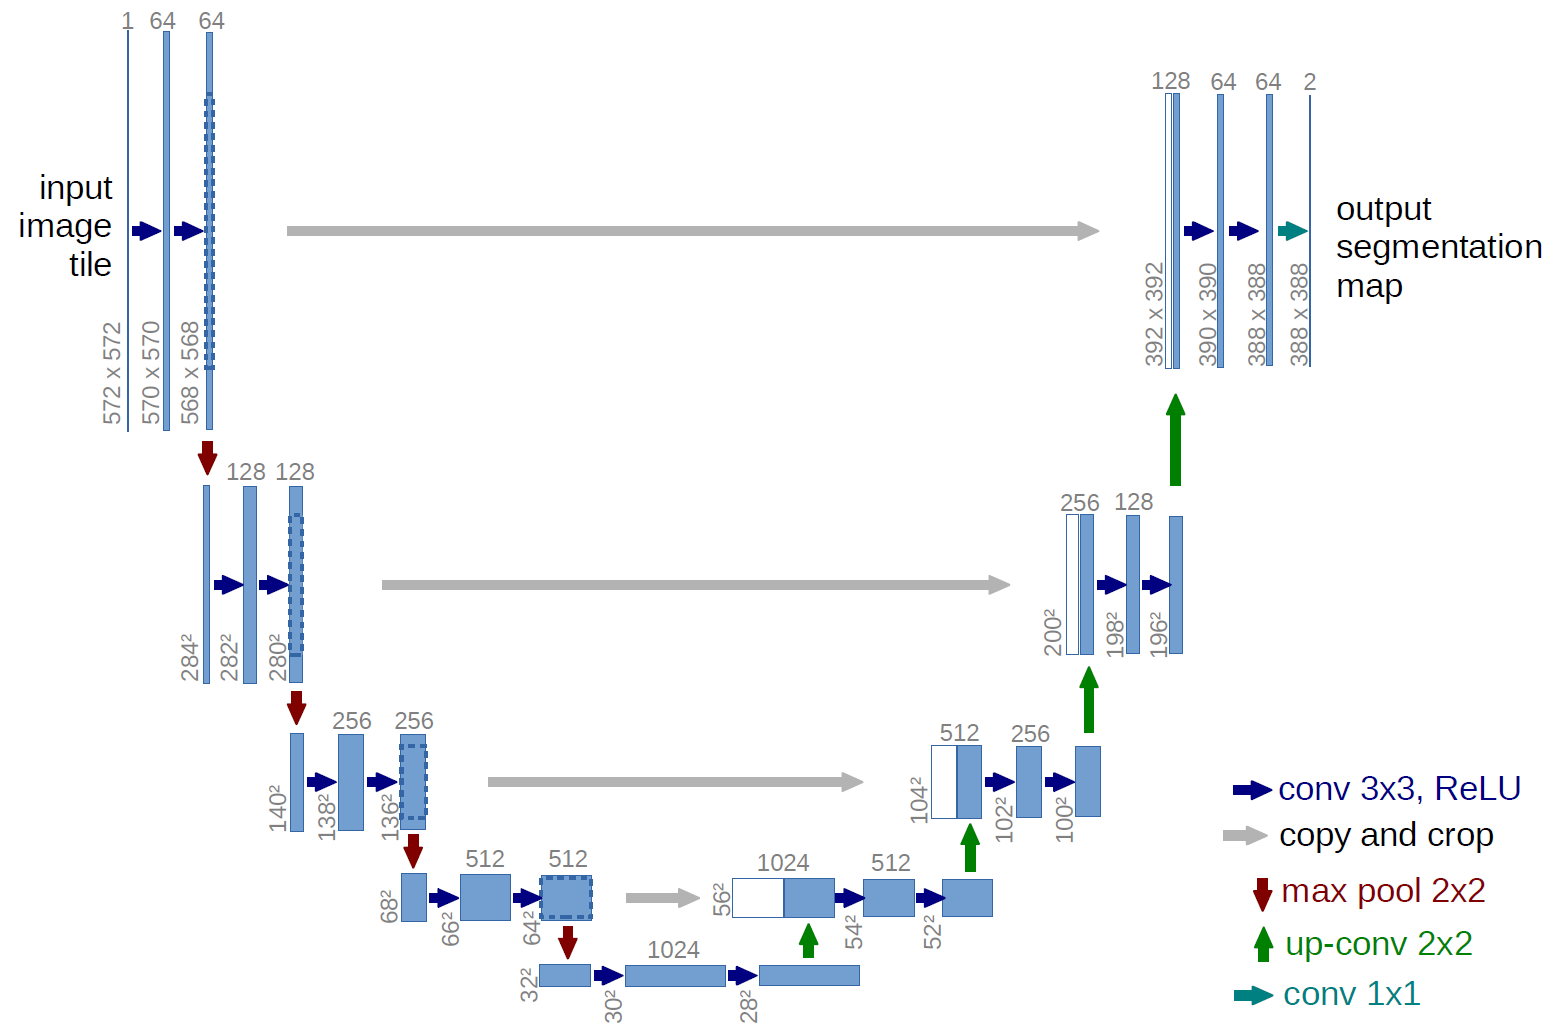
\includegraphics[width=0.6\textwidth]{./img/unet_architecture.png}
    \caption{UNet Architecture}
    \label{fig:unet_architecture}
\end{figure}

\section{Architecture}
The UNet architecture consists of two main parts: the encoder and the decoder. The encoder captures the context of the image, while the decoder enables precise localization. The architecture is symmetric, with skip connections that allow for better gradient flow and feature reuse.

\subsection{Dice Coeeficient}
The loss function used is the Dice coefficient, which is a measure of overlap between two samples. It is defined as:
\begin{equation}
    \text{Dice}(A, B) = \frac{2 |A \cap B|}{|A| + |B|}
\end{equation}
where \(A\) and \(B\) are the predicted and ground truth masks, respectively. The Dice coefficient ranges from 0 to 1, where 1 indicates perfect overlap.

However, the Dice coefficient was also used to calculate the accuracy of the model. The accuracy is defined as:
\begin{equation}
    \text{Accuracy} = \frac{TP + TN}{TP + TN + FP + FN}
\end{equation}
where \(TP\) is true positive, \(TN\) is true negative, \(FP\) is false positive, and \(FN\) is false negative.

Accuracy includes true negatives (correctly labeled background pixels), which often dominate in medical images (e.g., brain scans with small lesions). As a result, a model that labels every pixel as background can achieve high accuracy while completely missing lesions.

Dice ignores true negatives, focusing only on the overlap of the foreground object. This makes it much more sensitive to how well the model segments the structure of interest, especially when that structure occupies a small fraction of the image.

Therefore, the Dice coefficient is a better metric for evaluating the performance of the model in this case.

\section{First Training Loop}
\begin{table}[H]
    \centering
    \begin{tabular}{ll}
    \toprule
    \textbf{Parameter} & \textbf{Value} \\
    \midrule
    batch\_size   & 16 \\
    epochs        & 7 \\
    lr            & 0.0003 \\
    workers       & 0 \\
    image\_size   & 256 \\
    aug\_scale    & 0.05 \\
    aug\_angle    & 15 \\
    \bottomrule
    \end{tabular}
    \caption{Training 1 Configuration Parameters}
    \label{tab:args}
\end{table}
    
Running the training script takes a long time, arount 40 minutes per epoch. Therefore I limited the number of epochs to 7. As we can see from \autoref{fig:training_loss_1}, the loss plateaus after 800 steps (around 4 epochs)

\begin{figure}[H]
    \centering
    \begin{minipage}[t]{0.48\textwidth}
        \centering
        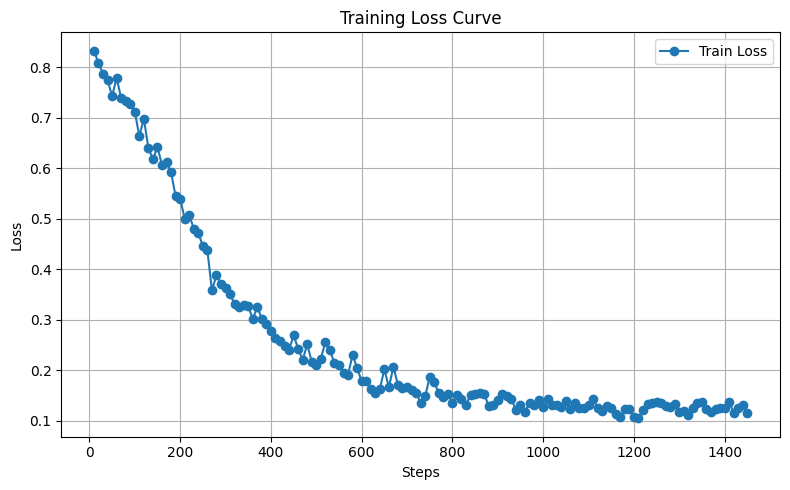
\includegraphics[width=\linewidth]{./img/training_loss_1.png}
        \caption{Loss over epochs (1)}
        \label{fig:training_loss_1}
    \end{minipage}
    \begin{minipage}[t]{0.48\textwidth}
        \centering
        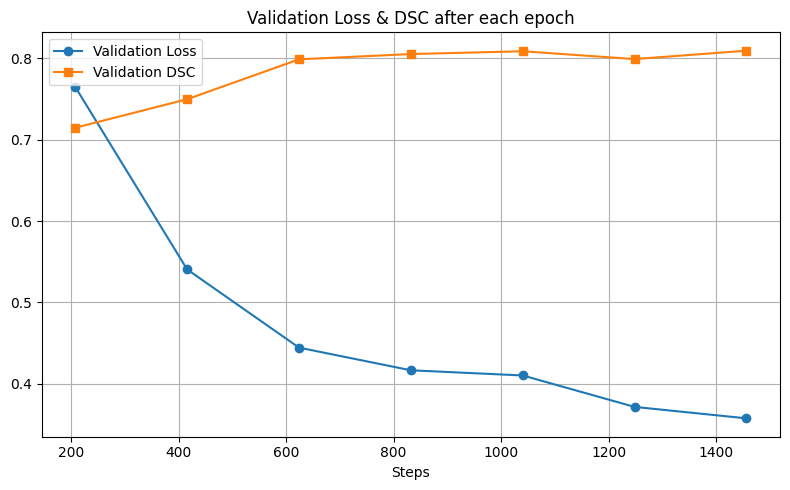
\includegraphics[width=\linewidth]{./img/validation_metric_per_epoch_1.png}
        \caption{Validation metrics per epoch (1)}
        \label{fig:validation_metric_per_epoch_1}
    \end{minipage}
\end{figure}

Moreover, \autoref{fig:validation_metric_per_epoch_1} shows the validation loss and DSC per epoch. This gives a better understanding of the model performance. We can see that the validation loss decreases much like over training, but its value is much higher than the training loss. This indicates that the model is overfitting to the training data. On the other hand, the validation DSC increases slightly in the beginning, but then fluctuates around 0.8.

To further evaluate the model, \autoref{fig:validation_accuracy} and \autoref{fig:validation_dsc} show accuracy and DSC metrics for the validation set. Each results are grouped by patients. The accuracy is greater than 0.98, which is very high. However, the DSC is only around 0.8. The red line represents the mean and the green line the median.

The patient \textit{3m\textbackslash TCGA\_CS\_6668} has a DSC score of 0, this is because the model predicted false positives in some images and could not identify the legion in other images.
\begin{figure}[H]
    \centering
    \begin{minipage}[t]{0.48\textwidth}
        \centering
        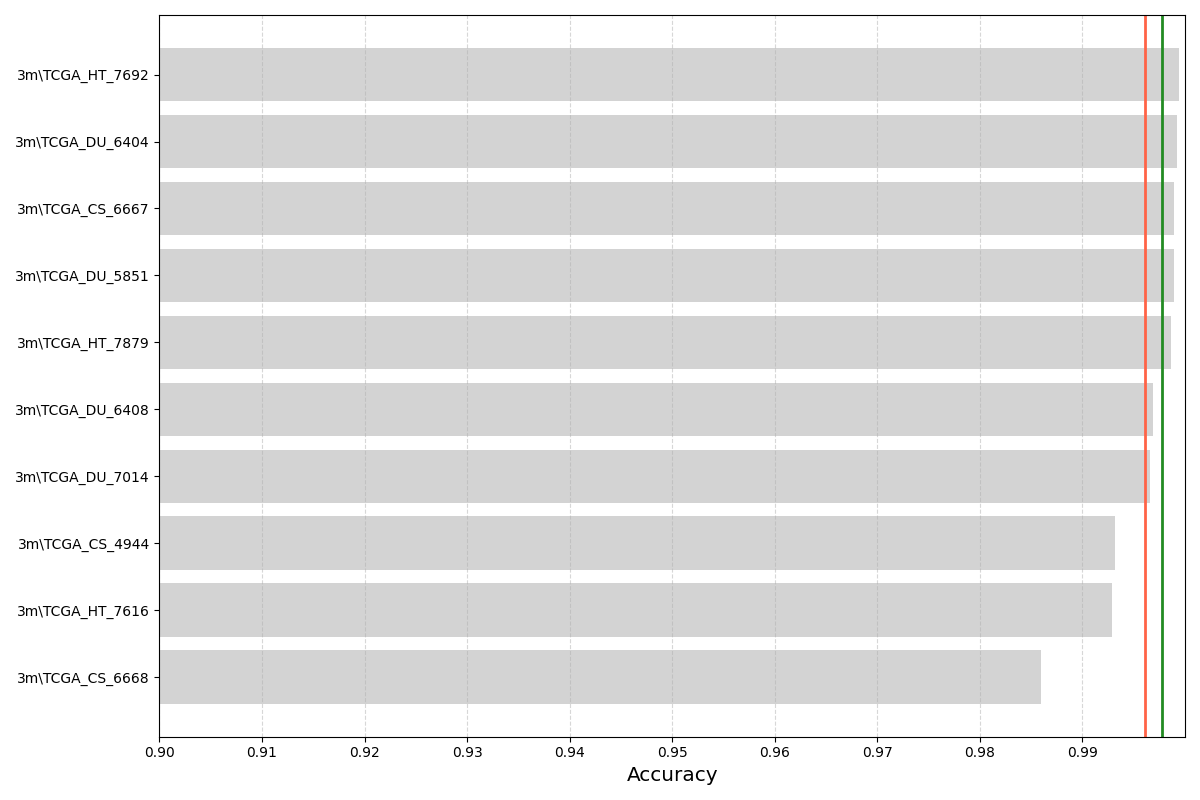
\includegraphics[width=\linewidth]{./img/validation_accuracy_1.png}
        \caption{Validation Accuracy}
        \label{fig:validation_accuracy}
    \end{minipage}
    \hfill
    \begin{minipage}[t]{0.48\textwidth}
        \centering
        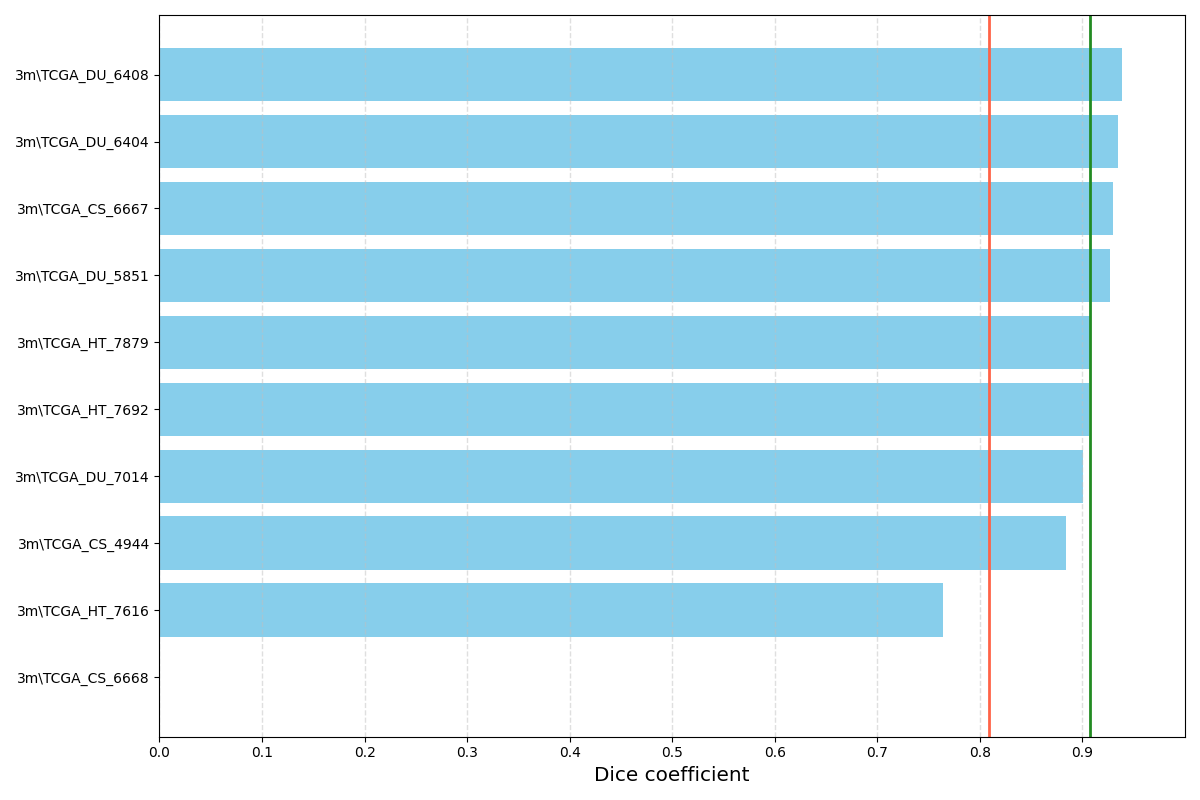
\includegraphics[width=\linewidth]{./img/validation_dsc_1.png}
        \caption{Validation DSC}
        \label{fig:validation_dsc}
    \end{minipage}
\end{figure}

\section{Second Training Loop}
\begin{table}[H]
    \centering
    \begin{tabular}{ll}
    \toprule
    \textbf{Parameter} & \textbf{Value} \\
    \midrule
    batch\_size   & 32 \\
    epochs        & 10 \\
    lr            & 0.001 \\
    wd            & 0.0001 \\
    workers       & 0 \\
    image\_size   & 256 \\
    aug\_scale    & 0.05 \\
    aug\_angle    & 15 \\
    \bottomrule
    \end{tabular}
    \caption{Training 2 Configuration Parameters}
    \label{tab:args_2}
\end{table}

For the second training lopp, I increased the batch size to 32 and the learning rate to 0.001. I also added weight decay to prevent overfitting. Training also took 40 minutes per epoch, so I limited it to 10 epochs this time.

The \autoref{fig:training_loss_2} shows that a higher learning rate leads to a faster convergence. The loss decreases much faster than in the first training loop. However, the loss plateaus at around 0.17 instead of 0.12. This indicates that the model is not able to learn as well as in the first training loop.

\begin{figure}[H]
    \centering
    \begin{minipage}[t]{0.48\textwidth}
        \centering
        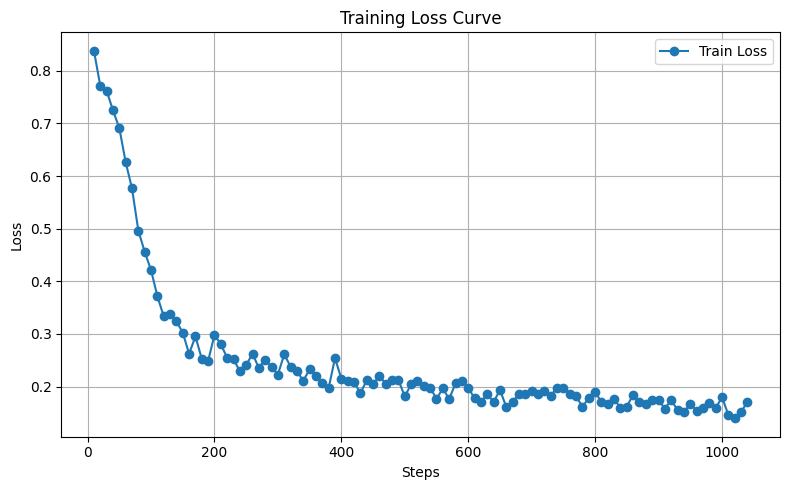
\includegraphics[width=\linewidth]{./img/training_loss_2.png}
        \caption{Loss over epochs (2)}
        \label{fig:training_loss_2}
    \end{minipage}
    \begin{minipage}[t]{0.48\textwidth}
        \centering
        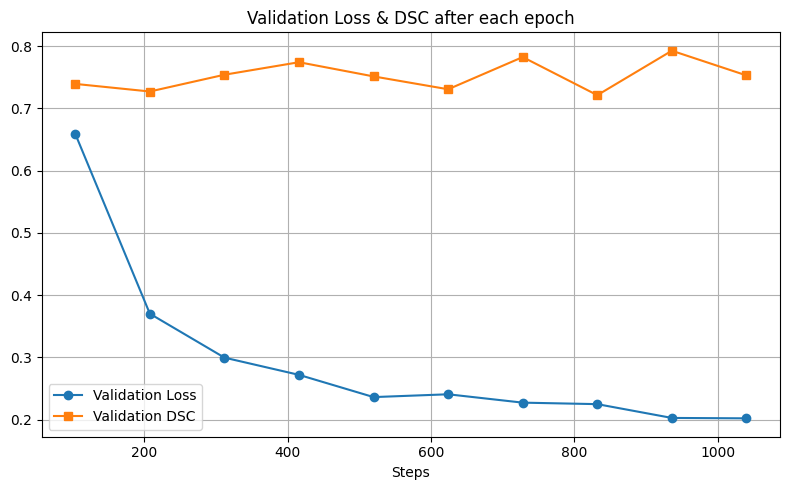
\includegraphics[width=\linewidth]{./img/validation_metric_per_epoch_2.png}
        \caption{Validation metrics per epoch (2)}
        \label{fig:validation_metric_per_epoch_2}
    \end{minipage}
\end{figure}

Next, here are the validation metrics per epoch. Compared to the first training loop, everything is slightly worse. For example, the mean DSC went from 0.8093 to 0.7925.

\begin{figure}[H]
    \centering
    \begin{minipage}[t]{0.48\textwidth}
        \centering
        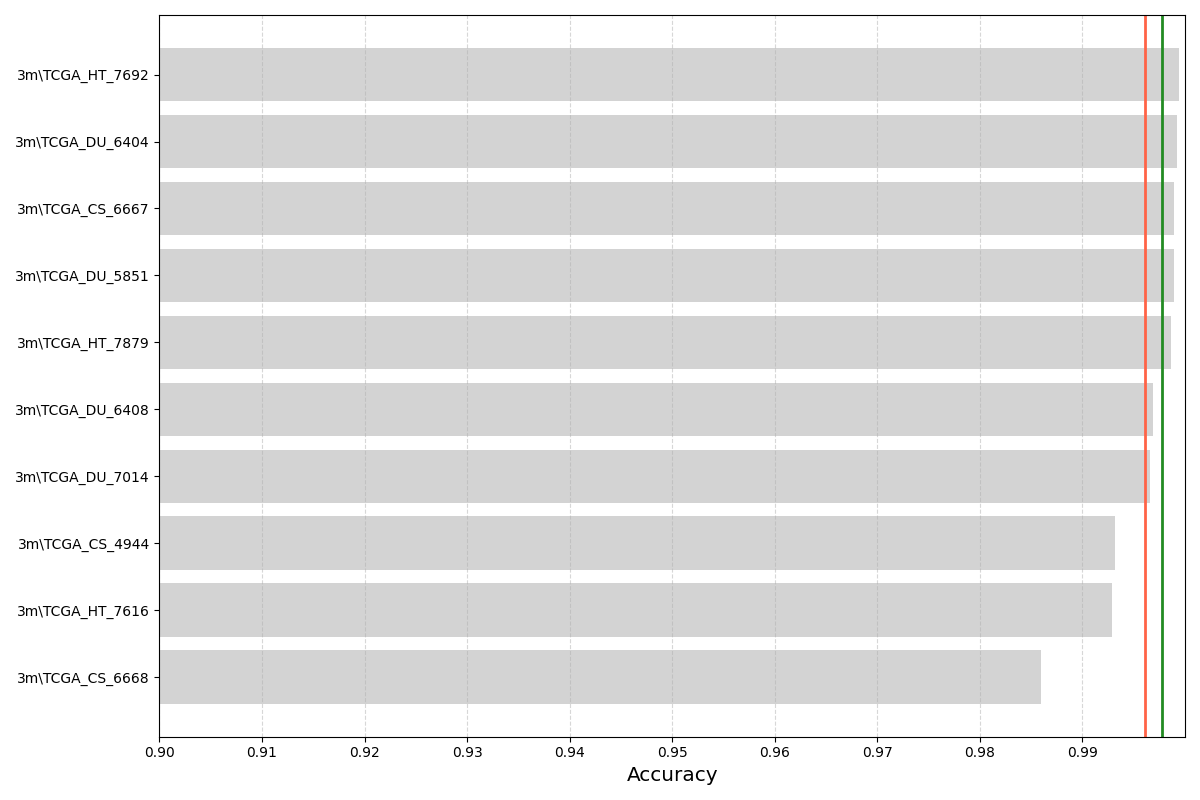
\includegraphics[width=\linewidth]{./img/validation_accuracy_2.png}
        \caption{Validation Accuracy (2)}
        \label{fig:validation_accuracy_2}
    \end{minipage}
    \hfill
    \begin{minipage}[t]{0.48\textwidth}
        \centering
        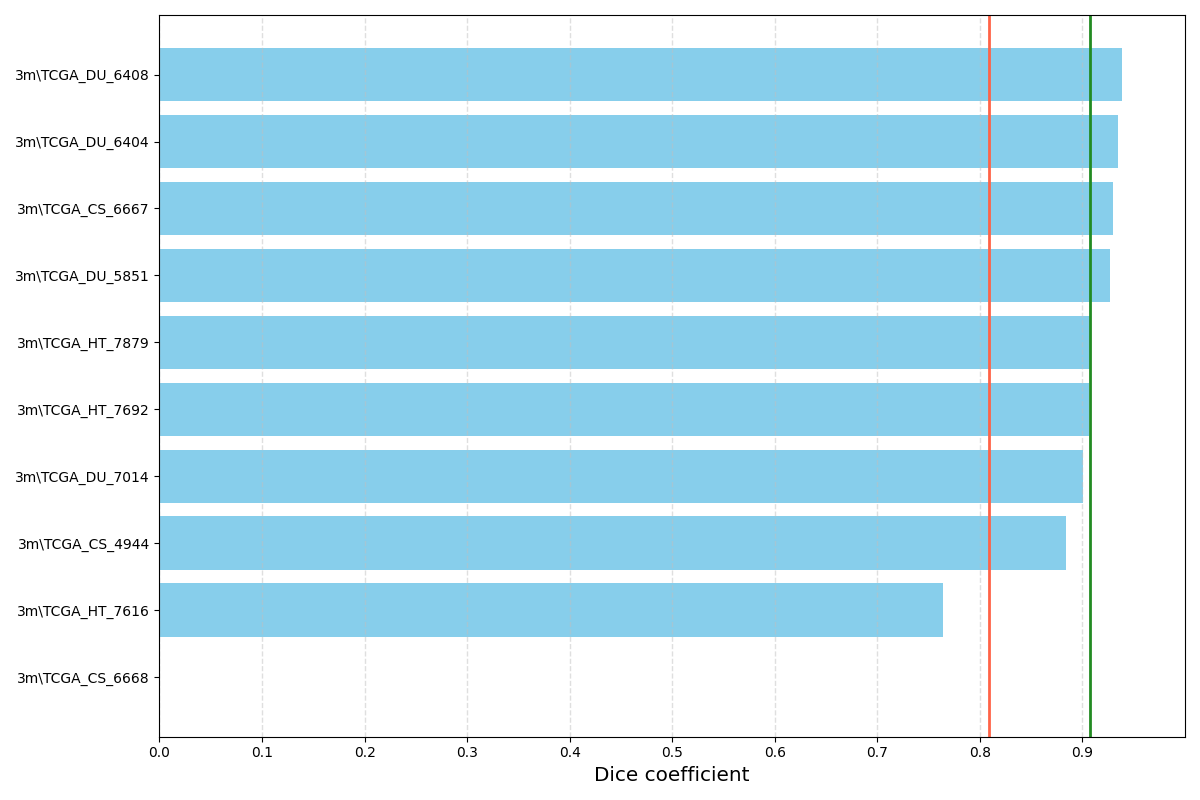
\includegraphics[width=\linewidth]{./img/validation_dsc_2.png}
        \caption{Validation DSC (2)}
        \label{fig:validation_dsc_2}
    \end{minipage}
\end{figure}

\section{Comparison}
The hyperparameters used in the first training loop were better than the second. And since the training time was very high, I changed many of them but now I am unable to see which one helped and which one worsened it.

\section{Results}
Here are some of the predictions made by the model, in red is the prediction and in green the ground truth. Both \autoref{fig:img_1} and \autoref{fig:img_2} are from the \textit{3m\textbackslash TCGA\_DU\_6408} patient, the one with the highest DSC score. We can see that the model is able to predict the legion quite well.

And both \autoref{fig:img_3} and \autoref{fig:img_4} are from the \textit{3m\textbackslash TCGA\_CS\_6668} patient, the one with the lowest DSC score. We can see that the model missed an area of legion and mistook the skull in upper sections of the brain for a legion.

\begin{figure}[H]
    \centering
    \begin{minipage}[t]{0.48\textwidth}
        \centering
        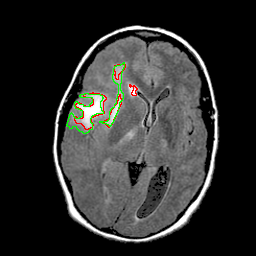
\includegraphics[width=\linewidth]{../predictions/kaggle_3m/TCGA_DU_6408_19860521-22.png}
        \caption{Prediction 1}
        \label{fig:img_1}
    \end{minipage}
    \hfill
    \begin{minipage}[t]{0.48\textwidth}
        \centering
        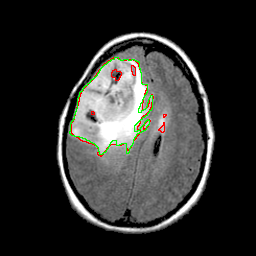
\includegraphics[width=\linewidth]{../predictions/kaggle_3m/TCGA_DU_6408_19860521-32.png}
        \caption{Prediction 2}
        \label{fig:img_2}
    \end{minipage}
\end{figure}

\begin{figure}[H]
    \centering
    \begin{minipage}[t]{0.48\textwidth}
        \centering
        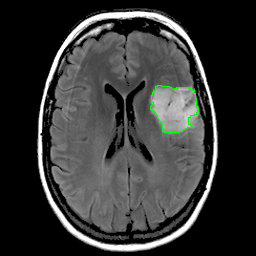
\includegraphics[width=\linewidth]{../predictions/kaggle_3m/TCGA_CS_6668_20011025-15.png}
        \caption{Prediction 3}
        \label{fig:img_3}
    \end{minipage}
    \hfill
    \begin{minipage}[t]{0.48\textwidth}
        \centering
        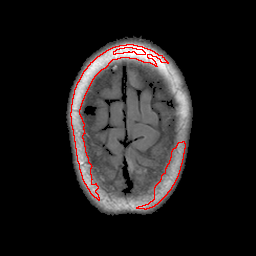
\includegraphics[width=\linewidth]{../predictions/kaggle_3m/TCGA_CS_6668_20011025-23.png}
        \caption{Prediction 4}
        \label{fig:img_4}
    \end{minipage}
\end{figure}

\begin{thebibliography}{9}
\bibitem{ronneberger2015u}
Ronneberger, O., Fischer, P., \& Brox, T. (2015). U-Net: Convolutional Networks for Biomedical Image Segmentation. \textit{Medical Image Computing and Computer-Assisted Intervention (MICCAI)}. \url{https://arxiv.org/abs/1505.04597}
\bibitem{kaggle}
Kaggle. (n.d.). Brain MRI dataset. Retrieved from \url{https://www.kaggle.com/mateuszbuda/lgg-mri-segmentation}
\end{thebibliography}

\end{document}